\documentclass[]{article}
\usepackage{lmodern}
\usepackage{amssymb,amsmath}
\usepackage{ifxetex,ifluatex}
\usepackage{fixltx2e} % provides \textsubscript
\ifnum 0\ifxetex 1\fi\ifluatex 1\fi=0 % if pdftex
  \usepackage[T1]{fontenc}
  \usepackage[utf8]{inputenc}
\else % if luatex or xelatex
  \ifxetex
    \usepackage{mathspec}
  \else
    \usepackage{fontspec}
  \fi
  \defaultfontfeatures{Ligatures=TeX,Scale=MatchLowercase}
\fi
% use upquote if available, for straight quotes in verbatim environments
\IfFileExists{upquote.sty}{\usepackage{upquote}}{}
% use microtype if available
\IfFileExists{microtype.sty}{%
\usepackage{microtype}
\UseMicrotypeSet[protrusion]{basicmath} % disable protrusion for tt fonts
}{}
\usepackage[margin=1in]{geometry}
\usepackage{hyperref}
\hypersetup{unicode=true,
            pdftitle={Exercises},
            pdfauthor={Bruna Wundervald},
            pdfborder={0 0 0},
            breaklinks=true}
\urlstyle{same}  % don't use monospace font for urls
\usepackage{color}
\usepackage{fancyvrb}
\newcommand{\VerbBar}{|}
\newcommand{\VERB}{\Verb[commandchars=\\\{\}]}
\DefineVerbatimEnvironment{Highlighting}{Verbatim}{commandchars=\\\{\}}
% Add ',fontsize=\small' for more characters per line
\usepackage{framed}
\definecolor{shadecolor}{RGB}{248,248,248}
\newenvironment{Shaded}{\begin{snugshade}}{\end{snugshade}}
\newcommand{\AlertTok}[1]{\textcolor[rgb]{0.94,0.16,0.16}{#1}}
\newcommand{\AnnotationTok}[1]{\textcolor[rgb]{0.56,0.35,0.01}{\textbf{\textit{#1}}}}
\newcommand{\AttributeTok}[1]{\textcolor[rgb]{0.77,0.63,0.00}{#1}}
\newcommand{\BaseNTok}[1]{\textcolor[rgb]{0.00,0.00,0.81}{#1}}
\newcommand{\BuiltInTok}[1]{#1}
\newcommand{\CharTok}[1]{\textcolor[rgb]{0.31,0.60,0.02}{#1}}
\newcommand{\CommentTok}[1]{\textcolor[rgb]{0.56,0.35,0.01}{\textit{#1}}}
\newcommand{\CommentVarTok}[1]{\textcolor[rgb]{0.56,0.35,0.01}{\textbf{\textit{#1}}}}
\newcommand{\ConstantTok}[1]{\textcolor[rgb]{0.00,0.00,0.00}{#1}}
\newcommand{\ControlFlowTok}[1]{\textcolor[rgb]{0.13,0.29,0.53}{\textbf{#1}}}
\newcommand{\DataTypeTok}[1]{\textcolor[rgb]{0.13,0.29,0.53}{#1}}
\newcommand{\DecValTok}[1]{\textcolor[rgb]{0.00,0.00,0.81}{#1}}
\newcommand{\DocumentationTok}[1]{\textcolor[rgb]{0.56,0.35,0.01}{\textbf{\textit{#1}}}}
\newcommand{\ErrorTok}[1]{\textcolor[rgb]{0.64,0.00,0.00}{\textbf{#1}}}
\newcommand{\ExtensionTok}[1]{#1}
\newcommand{\FloatTok}[1]{\textcolor[rgb]{0.00,0.00,0.81}{#1}}
\newcommand{\FunctionTok}[1]{\textcolor[rgb]{0.00,0.00,0.00}{#1}}
\newcommand{\ImportTok}[1]{#1}
\newcommand{\InformationTok}[1]{\textcolor[rgb]{0.56,0.35,0.01}{\textbf{\textit{#1}}}}
\newcommand{\KeywordTok}[1]{\textcolor[rgb]{0.13,0.29,0.53}{\textbf{#1}}}
\newcommand{\NormalTok}[1]{#1}
\newcommand{\OperatorTok}[1]{\textcolor[rgb]{0.81,0.36,0.00}{\textbf{#1}}}
\newcommand{\OtherTok}[1]{\textcolor[rgb]{0.56,0.35,0.01}{#1}}
\newcommand{\PreprocessorTok}[1]{\textcolor[rgb]{0.56,0.35,0.01}{\textit{#1}}}
\newcommand{\RegionMarkerTok}[1]{#1}
\newcommand{\SpecialCharTok}[1]{\textcolor[rgb]{0.00,0.00,0.00}{#1}}
\newcommand{\SpecialStringTok}[1]{\textcolor[rgb]{0.31,0.60,0.02}{#1}}
\newcommand{\StringTok}[1]{\textcolor[rgb]{0.31,0.60,0.02}{#1}}
\newcommand{\VariableTok}[1]{\textcolor[rgb]{0.00,0.00,0.00}{#1}}
\newcommand{\VerbatimStringTok}[1]{\textcolor[rgb]{0.31,0.60,0.02}{#1}}
\newcommand{\WarningTok}[1]{\textcolor[rgb]{0.56,0.35,0.01}{\textbf{\textit{#1}}}}
\usepackage{graphicx,grffile}
\makeatletter
\def\maxwidth{\ifdim\Gin@nat@width>\linewidth\linewidth\else\Gin@nat@width\fi}
\def\maxheight{\ifdim\Gin@nat@height>\textheight\textheight\else\Gin@nat@height\fi}
\makeatother
% Scale images if necessary, so that they will not overflow the page
% margins by default, and it is still possible to overwrite the defaults
% using explicit options in \includegraphics[width, height, ...]{}
\setkeys{Gin}{width=\maxwidth,height=\maxheight,keepaspectratio}
\IfFileExists{parskip.sty}{%
\usepackage{parskip}
}{% else
\setlength{\parindent}{0pt}
\setlength{\parskip}{6pt plus 2pt minus 1pt}
}
\setlength{\emergencystretch}{3em}  % prevent overfull lines
\providecommand{\tightlist}{%
  \setlength{\itemsep}{0pt}\setlength{\parskip}{0pt}}
\setcounter{secnumdepth}{0}
% Redefines (sub)paragraphs to behave more like sections
\ifx\paragraph\undefined\else
\let\oldparagraph\paragraph
\renewcommand{\paragraph}[1]{\oldparagraph{#1}\mbox{}}
\fi
\ifx\subparagraph\undefined\else
\let\oldsubparagraph\subparagraph
\renewcommand{\subparagraph}[1]{\oldsubparagraph{#1}\mbox{}}
\fi

%%% Use protect on footnotes to avoid problems with footnotes in titles
\let\rmarkdownfootnote\footnote%
\def\footnote{\protect\rmarkdownfootnote}

%%% Change title format to be more compact
\usepackage{titling}

% Create subtitle command for use in maketitle
\newcommand{\subtitle}[1]{
  \posttitle{
    \begin{center}\large#1\end{center}
    }
}

\setlength{\droptitle}{-2em}

  \title{Exercises}
    \pretitle{\vspace{\droptitle}\centering\huge}
  \posttitle{\par}
    \author{Bruna Wundervald}
    \preauthor{\centering\large\emph}
  \postauthor{\par}
      \predate{\centering\large\emph}
  \postdate{\par}
    \date{April, 2019}


\begin{document}
\maketitle

\begin{Shaded}
\begin{Highlighting}[]
\KeywordTok{set.seed}\NormalTok{(}\DecValTok{2019}\NormalTok{)}
\NormalTok{B <-}\StringTok{ }\DecValTok{1000}
\NormalTok{n <-}\StringTok{ }\DecValTok{25}
\NormalTok{M <-}\StringTok{ }\DecValTok{3}
\NormalTok{pmax <-}\StringTok{ }\DecValTok{20}

\NormalTok{x <-}\StringTok{ }\KeywordTok{rep}\NormalTok{(}\KeywordTok{seq}\NormalTok{(}\DataTypeTok{from =} \DecValTok{-10}\NormalTok{, }\DataTypeTok{to =} \DecValTok{10}\NormalTok{, }\DataTypeTok{length =}\NormalTok{ n), }\DataTypeTok{each =}\NormalTok{ M)}

\NormalTok{w <-}\StringTok{ }\ControlFlowTok{function}\NormalTok{(x)\{}
  \FloatTok{0.001} \OperatorTok{*}\StringTok{ }\NormalTok{(}\DecValTok{100} \OperatorTok{+}\StringTok{ }\NormalTok{x }\OperatorTok{+}\StringTok{ }\NormalTok{x}\OperatorTok{^}\DecValTok{2} \OperatorTok{+}\StringTok{ }\NormalTok{x}\OperatorTok{^}\StringTok{ }\DecValTok{3}\NormalTok{)}
\NormalTok{\}}

\NormalTok{mu <-}\StringTok{ }\ControlFlowTok{function}\NormalTok{(x) \{}
  \DecValTok{8} \OperatorTok{*}\StringTok{ }\KeywordTok{exp}\NormalTok{(}\KeywordTok{w}\NormalTok{(x))}
\NormalTok{\}}

\NormalTok{aics <-}\StringTok{ }\KeywordTok{matrix}\NormalTok{(}\DecValTok{0}\NormalTok{, }\DataTypeTok{nrow =}\NormalTok{ B, }\DataTypeTok{ncol =}\NormalTok{ pmax)}


\ControlFlowTok{for}\NormalTok{(b }\ControlFlowTok{in} \DecValTok{1}\OperatorTok{:}\NormalTok{B)\{}
  
\NormalTok{  y <-}\StringTok{ }\KeywordTok{rpois}\NormalTok{(}\DataTypeTok{n =}\NormalTok{ M }\OperatorTok{*}\StringTok{ }\NormalTok{n, }\DataTypeTok{lambda =} \KeywordTok{mu}\NormalTok{(x))}
  
\NormalTok{  mod <-}\StringTok{ }\KeywordTok{glm}\NormalTok{(y }\OperatorTok{~}\StringTok{ }\DecValTok{1}\NormalTok{, }\DataTypeTok{family =}\NormalTok{ poisson)}
\NormalTok{  aics[b, }\DecValTok{1}\NormalTok{] <-}\StringTok{ }\KeywordTok{AIC}\NormalTok{(mod)}
  
\NormalTok{  formula <-}\StringTok{ "y ~ x"}
\NormalTok{  mod <-}\StringTok{ }\KeywordTok{glm}\NormalTok{(formula, }\DataTypeTok{family =}\NormalTok{ poisson)}
\NormalTok{  aics[b, }\DecValTok{2}\NormalTok{ ] <-}\StringTok{ }\KeywordTok{AIC}\NormalTok{(mod)}
  
  \ControlFlowTok{for}\NormalTok{(j }\ControlFlowTok{in} \DecValTok{3}\OperatorTok{:}\NormalTok{pmax)\{}
\NormalTok{    formula <-}\StringTok{ }\KeywordTok{paste}\NormalTok{(formula, }\StringTok{" + I(x^"}\NormalTok{, j }\OperatorTok{-}\StringTok{ }\DecValTok{1}\NormalTok{, }\StringTok{")"}\NormalTok{, }\DataTypeTok{sep =} \StringTok{""}\NormalTok{)}
\NormalTok{    mod <-}\StringTok{ }\KeywordTok{glm}\NormalTok{(formula, }\DataTypeTok{family =}\NormalTok{ poisson)}
\NormalTok{    aics[b, j] <-}\StringTok{ }\KeywordTok{AIC}\NormalTok{(mod)}
\NormalTok{  \}}
\NormalTok{\}}

\NormalTok{AICorder <-}\StringTok{ }\KeywordTok{apply}\NormalTok{(aics, }\DecValTok{1}\NormalTok{, which.min) }\OperatorTok{-}\StringTok{ }\DecValTok{1}
\NormalTok{tAIC <-}\StringTok{ }\KeywordTok{table}\NormalTok{(AICorder)}
\end{Highlighting}
\end{Shaded}

\begin{Shaded}
\begin{Highlighting}[]
\NormalTok{tAIC }\OperatorTok\StringTok{ }
\StringTok{  }\KeywordTok{as.data.frame}\NormalTok{() }\OperatorTok\StringTok{ }
\StringTok{  }\KeywordTok{ggplot}\NormalTok{(}\KeywordTok{aes}\NormalTok{(AICorder, Freq, }\DataTypeTok{group =} \DecValTok{1}\NormalTok{)) }\OperatorTok{+}
\StringTok{  }\KeywordTok{geom_line}\NormalTok{(}\DataTypeTok{colour =} \StringTok{"gray80"}\NormalTok{) }\OperatorTok{+}
\StringTok{  }\KeywordTok{geom_point}\NormalTok{(}\DataTypeTok{colour =} \StringTok{"plum"}\NormalTok{) }\OperatorTok{+}
\StringTok{  }\KeywordTok{theme_bw}\NormalTok{()}
\end{Highlighting}
\end{Shaded}

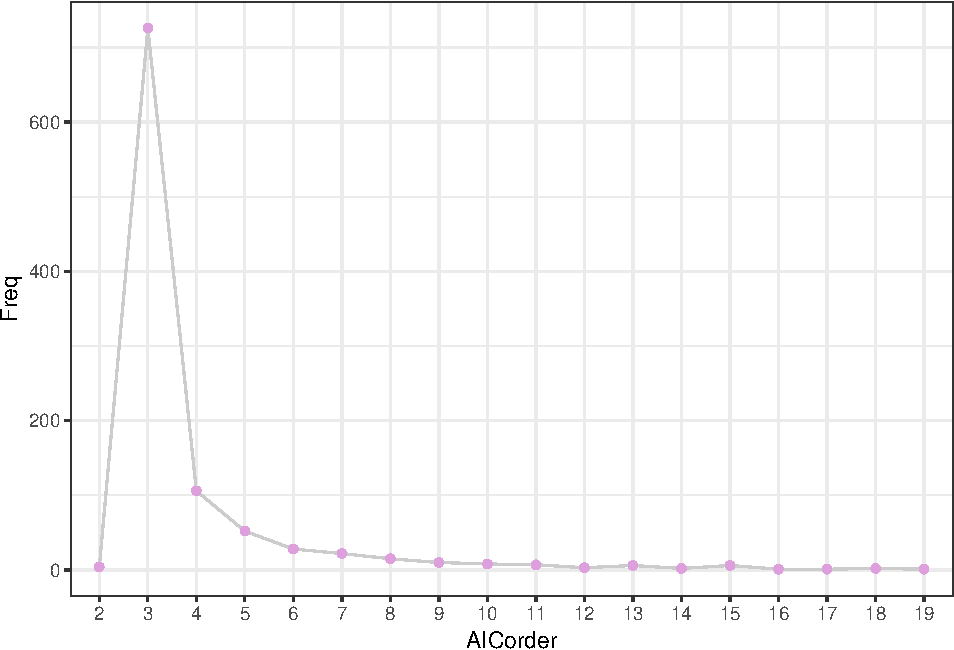
\includegraphics{exercises_files/figure-latex/unnamed-chunk-2-1.pdf}

\begin{enumerate}
\def\labelenumi{\arabic{enumi}.}
\tightlist
\item
  Investigate the performance of AIC as a model selection tool for
  \(n=25, 50, 100, 1000\).
\end{enumerate}

\begin{Shaded}
\begin{Highlighting}[]
\NormalTok{x_sim <-}\StringTok{ }\KeywordTok{c}\NormalTok{(}\DecValTok{25}\NormalTok{, }\DecValTok{50}\NormalTok{, }\DecValTok{100}\NormalTok{, }\DecValTok{1000}\NormalTok{) }\OperatorTok\StringTok{ }
\StringTok{  }\NormalTok{purrr}\OperatorTok{::}\KeywordTok{map}\NormalTok{(}\OperatorTok{~}\NormalTok{\{}
    \KeywordTok{rep}\NormalTok{(}\KeywordTok{seq}\NormalTok{(}\DataTypeTok{from =} \DecValTok{-10}\NormalTok{, }\DataTypeTok{to =} \DecValTok{10}\NormalTok{, }\DataTypeTok{length =}\NormalTok{ .x), }\DataTypeTok{each =}\NormalTok{ M)  }
\NormalTok{  \})}

\CommentTok{#-------}
\ControlFlowTok{for}\NormalTok{(b }\ControlFlowTok{in} \DecValTok{1}\OperatorTok{:}\NormalTok{B)\{}
  
\NormalTok{  y <-}\StringTok{ }\KeywordTok{rpois}\NormalTok{(}\DataTypeTok{n =}\NormalTok{ M }\OperatorTok{*}\StringTok{ }\NormalTok{n, }\DataTypeTok{lambda =} \KeywordTok{mu}\NormalTok{(x_sim[[}\DecValTok{1}\NormalTok{]]))}
  
\NormalTok{  mod <-}\StringTok{ }\KeywordTok{glm}\NormalTok{(y }\OperatorTok{~}\StringTok{ }\DecValTok{1}\NormalTok{, }\DataTypeTok{family =}\NormalTok{ poisson)}
\NormalTok{  aics[b, }\DecValTok{1}\NormalTok{] <-}\StringTok{ }\KeywordTok{AIC}\NormalTok{(mod)}
  
\NormalTok{  formula <-}\StringTok{ "y ~ x"}
\NormalTok{  mod <-}\StringTok{ }\KeywordTok{glm}\NormalTok{(formula, }\DataTypeTok{family =}\NormalTok{ poisson)}
\NormalTok{  aics[b, }\DecValTok{2}\NormalTok{ ] <-}\StringTok{ }\KeywordTok{AIC}\NormalTok{(mod)}
  
  \ControlFlowTok{for}\NormalTok{(j }\ControlFlowTok{in} \DecValTok{3}\OperatorTok{:}\NormalTok{pmax)\{}
\NormalTok{    formula <-}\StringTok{ }\KeywordTok{paste}\NormalTok{(formula, }\StringTok{" + I(x^"}\NormalTok{, j }\OperatorTok{-}\StringTok{ }\DecValTok{1}\NormalTok{, }\StringTok{")"}\NormalTok{, }\DataTypeTok{sep =} \StringTok{""}\NormalTok{)}
\NormalTok{    mod <-}\StringTok{ }\KeywordTok{glm}\NormalTok{(formula, }\DataTypeTok{family =}\NormalTok{ poisson)}
\NormalTok{    aics[b, j] <-}\StringTok{ }\KeywordTok{AIC}\NormalTok{(mod)}
\NormalTok{  \}}
\NormalTok{\}}

\NormalTok{AICorder_}\DecValTok{25}\NormalTok{ <-}\StringTok{ }\KeywordTok{apply}\NormalTok{(aics, }\DecValTok{1}\NormalTok{, which.min) }\OperatorTok{-}\StringTok{ }\DecValTok{1}
\NormalTok{tAIC_}\DecValTok{25}\NormalTok{ <-}\StringTok{ }\KeywordTok{table}\NormalTok{(AICorder_}\DecValTok{25}\NormalTok{)}
\NormalTok{tAIC_}\DecValTok{25}
\end{Highlighting}
\end{Shaded}

\begin{verbatim}
## AICorder_25
##   2   3   4   5   6   7   8   9  10  11  12  13  14  15  16  17  18  19 
##   2 694 112  55  43  24  16  16   8   6   7   4   3   2   4   1   2   1
\end{verbatim}

\begin{Shaded}
\begin{Highlighting}[]
\CommentTok{#-------}
\ControlFlowTok{for}\NormalTok{(b }\ControlFlowTok{in} \DecValTok{1}\OperatorTok{:}\NormalTok{B)\{}
  
\NormalTok{  y <-}\StringTok{ }\KeywordTok{rpois}\NormalTok{(}\DataTypeTok{n =}\NormalTok{ M }\OperatorTok{*}\StringTok{ }\NormalTok{n, }\DataTypeTok{lambda =} \KeywordTok{mu}\NormalTok{(x_sim[[}\DecValTok{2}\NormalTok{]]))}
  
\NormalTok{  mod <-}\StringTok{ }\KeywordTok{glm}\NormalTok{(y }\OperatorTok{~}\StringTok{ }\DecValTok{1}\NormalTok{, }\DataTypeTok{family =}\NormalTok{ poisson)}
\NormalTok{  aics[b, }\DecValTok{1}\NormalTok{] <-}\StringTok{ }\KeywordTok{AIC}\NormalTok{(mod)}
  
\NormalTok{  formula <-}\StringTok{ "y ~ x"}
\NormalTok{  mod <-}\StringTok{ }\KeywordTok{glm}\NormalTok{(formula, }\DataTypeTok{family =}\NormalTok{ poisson)}
\NormalTok{  aics[b, }\DecValTok{2}\NormalTok{ ] <-}\StringTok{ }\KeywordTok{AIC}\NormalTok{(mod)}
  
  \ControlFlowTok{for}\NormalTok{(j }\ControlFlowTok{in} \DecValTok{3}\OperatorTok{:}\NormalTok{pmax)\{}
\NormalTok{    formula <-}\StringTok{ }\KeywordTok{paste}\NormalTok{(formula, }\StringTok{" + I(x^"}\NormalTok{, j }\OperatorTok{-}\StringTok{ }\DecValTok{1}\NormalTok{, }\StringTok{")"}\NormalTok{, }\DataTypeTok{sep =} \StringTok{""}\NormalTok{)}
\NormalTok{    mod <-}\StringTok{ }\KeywordTok{glm}\NormalTok{(formula, }\DataTypeTok{family =}\NormalTok{ poisson)}
\NormalTok{    aics[b, j] <-}\StringTok{ }\KeywordTok{AIC}\NormalTok{(mod)}
\NormalTok{  \}}
\NormalTok{\}}
\NormalTok{AICorder_}\DecValTok{50}\NormalTok{ <-}\StringTok{ }\KeywordTok{apply}\NormalTok{(aics, }\DecValTok{1}\NormalTok{, which.min) }\OperatorTok{-}\StringTok{ }\DecValTok{1}
\NormalTok{tAIC_}\DecValTok{50}\NormalTok{ <-}\StringTok{ }\KeywordTok{table}\NormalTok{(AICorder_}\DecValTok{50}\NormalTok{)}
\NormalTok{tAIC_}\DecValTok{50}
\end{Highlighting}
\end{Shaded}

\begin{verbatim}
## AICorder_50
##   1   2   3   4   5   6   7   8   9  10  11  12  13  14  15  17  18  19 
## 110 579 132  57  27  23  13  21   8   6   5   5   4   3   2   2   1   2
\end{verbatim}

\begin{Shaded}
\begin{Highlighting}[]
\CommentTok{#-------}
\ControlFlowTok{for}\NormalTok{(b }\ControlFlowTok{in} \DecValTok{1}\OperatorTok{:}\NormalTok{B)\{}
  
\NormalTok{  y <-}\StringTok{ }\KeywordTok{rpois}\NormalTok{(}\DataTypeTok{n =}\NormalTok{ M }\OperatorTok{*}\StringTok{ }\NormalTok{n, }\DataTypeTok{lambda =} \KeywordTok{mu}\NormalTok{(x_sim[[}\DecValTok{3}\NormalTok{]]))}
  
\NormalTok{  mod <-}\StringTok{ }\KeywordTok{glm}\NormalTok{(y }\OperatorTok{~}\StringTok{ }\DecValTok{1}\NormalTok{, }\DataTypeTok{family =}\NormalTok{ poisson)}
\NormalTok{  aics[b, }\DecValTok{1}\NormalTok{] <-}\StringTok{ }\KeywordTok{AIC}\NormalTok{(mod)}
  
\NormalTok{  formula <-}\StringTok{ "y ~ x"}
\NormalTok{  mod <-}\StringTok{ }\KeywordTok{glm}\NormalTok{(formula, }\DataTypeTok{family =}\NormalTok{ poisson)}
\NormalTok{  aics[b, }\DecValTok{2}\NormalTok{ ] <-}\StringTok{ }\KeywordTok{AIC}\NormalTok{(mod)}
  
  \ControlFlowTok{for}\NormalTok{(j }\ControlFlowTok{in} \DecValTok{3}\OperatorTok{:}\NormalTok{pmax)\{}
\NormalTok{    formula <-}\StringTok{ }\KeywordTok{paste}\NormalTok{(formula, }\StringTok{" + I(x^"}\NormalTok{, j }\OperatorTok{-}\StringTok{ }\DecValTok{1}\NormalTok{, }\StringTok{")"}\NormalTok{, }\DataTypeTok{sep =} \StringTok{""}\NormalTok{)}
\NormalTok{    mod <-}\StringTok{ }\KeywordTok{glm}\NormalTok{(formula, }\DataTypeTok{family =}\NormalTok{ poisson)}
\NormalTok{    aics[b, j] <-}\StringTok{ }\KeywordTok{AIC}\NormalTok{(mod)}
\NormalTok{  \}}
\NormalTok{\}}
\NormalTok{AICorder_}\DecValTok{100}\NormalTok{ <-}\StringTok{ }\KeywordTok{apply}\NormalTok{(aics, }\DecValTok{1}\NormalTok{, which.min) }\OperatorTok{-}\StringTok{ }\DecValTok{1}
\NormalTok{tAIC_}\DecValTok{100}\NormalTok{ <-}\StringTok{ }\KeywordTok{table}\NormalTok{(AICorder_}\DecValTok{100}\NormalTok{)}
\NormalTok{tAIC_}\DecValTok{100}
\end{Highlighting}
\end{Shaded}

\begin{verbatim}
## AICorder_100
##   0   1   2   3   4   5   6   7   8   9  10  11  12  13  14  16 
##   1 615 180  68  46  21  17  14   9   6   9   4   6   2   1   1
\end{verbatim}

\begin{Shaded}
\begin{Highlighting}[]
\CommentTok{#-------}
\ControlFlowTok{for}\NormalTok{(b }\ControlFlowTok{in} \DecValTok{1}\OperatorTok{:}\NormalTok{B)\{}
  
\NormalTok{  y <-}\StringTok{ }\KeywordTok{rpois}\NormalTok{(}\DataTypeTok{n =}\NormalTok{ M }\OperatorTok{*}\StringTok{ }\NormalTok{n, }\DataTypeTok{lambda =} \KeywordTok{mu}\NormalTok{(x_sim[[}\DecValTok{3}\NormalTok{]]))}
  
\NormalTok{  mod <-}\StringTok{ }\KeywordTok{glm}\NormalTok{(y }\OperatorTok{~}\StringTok{ }\DecValTok{1}\NormalTok{, }\DataTypeTok{family =}\NormalTok{ poisson)}
\NormalTok{  aics[b, }\DecValTok{1}\NormalTok{] <-}\StringTok{ }\KeywordTok{AIC}\NormalTok{(mod)}
  
\NormalTok{  formula <-}\StringTok{ "y ~ x"}
\NormalTok{  mod <-}\StringTok{ }\KeywordTok{glm}\NormalTok{(formula, }\DataTypeTok{family =}\NormalTok{ poisson)}
\NormalTok{  aics[b, }\DecValTok{2}\NormalTok{ ] <-}\StringTok{ }\KeywordTok{AIC}\NormalTok{(mod)}
  
  \ControlFlowTok{for}\NormalTok{(j }\ControlFlowTok{in} \DecValTok{3}\OperatorTok{:}\NormalTok{pmax)\{}
\NormalTok{    formula <-}\StringTok{ }\KeywordTok{paste}\NormalTok{(formula, }\StringTok{" + I(x^"}\NormalTok{, j }\OperatorTok{-}\StringTok{ }\DecValTok{1}\NormalTok{, }\StringTok{")"}\NormalTok{, }\DataTypeTok{sep =} \StringTok{""}\NormalTok{)}
\NormalTok{    mod <-}\StringTok{ }\KeywordTok{glm}\NormalTok{(formula, }\DataTypeTok{family =}\NormalTok{ poisson)}
\NormalTok{    aics[b, j] <-}\StringTok{ }\KeywordTok{AIC}\NormalTok{(mod)}
\NormalTok{  \}}
\NormalTok{\}}

\NormalTok{AICorder_}\DecValTok{1000}\NormalTok{ <-}\StringTok{ }\KeywordTok{apply}\NormalTok{(aics, }\DecValTok{1}\NormalTok{, which.min) }\OperatorTok{-}\StringTok{ }\DecValTok{1}
\NormalTok{tAIC_}\DecValTok{1000}\NormalTok{ <-}\StringTok{ }\KeywordTok{table}\NormalTok{(AICorder_}\DecValTok{1000}\NormalTok{)}
\NormalTok{tAIC_}\DecValTok{1000}
\end{Highlighting}
\end{Shaded}

\begin{verbatim}
## AICorder_1000
##   1   2   3   4   5   6   7   8   9  10  11  12  13  14  15  17  19 
## 594 220  57  45  20  16  13   5   8   3   6   4   4   2   1   1   1
\end{verbatim}

\begin{Shaded}
\begin{Highlighting}[]
\CommentTok{#--------}

\KeywordTok{cbind}\NormalTok{(tAIC_}\DecValTok{25}\NormalTok{, tAIC_}\DecValTok{50}\NormalTok{, tAIC_}\DecValTok{100}\NormalTok{, tAIC_}\DecValTok{1000}\NormalTok{) }\OperatorTok
\StringTok{  }\KeywordTok{as.data.frame}\NormalTok{() }\OperatorTok\StringTok{ }
\StringTok{  }\KeywordTok{gather}\NormalTok{() }\OperatorTok\StringTok{ }
\StringTok{   }\KeywordTok{mutate}\NormalTok{(}\DataTypeTok{pars =} \KeywordTok{rep}\NormalTok{(}\DecValTok{1}\OperatorTok{:}\DecValTok{18}\NormalTok{,  }\DecValTok{4}\NormalTok{)) }\OperatorTok\StringTok{ }
\StringTok{  }\KeywordTok{ggplot}\NormalTok{(}\KeywordTok{aes}\NormalTok{(pars, value, }\DataTypeTok{group =} \DecValTok{1}\NormalTok{)) }\OperatorTok{+}
\StringTok{  }\KeywordTok{geom_line}\NormalTok{(}\DataTypeTok{colour =} \StringTok{"gray80"}\NormalTok{) }\OperatorTok{+}
\StringTok{  }\KeywordTok{geom_point}\NormalTok{(}\DataTypeTok{colour =} \StringTok{"tomato"}\NormalTok{) }\OperatorTok{+}
\StringTok{  }\KeywordTok{facet_wrap}\NormalTok{(}\OperatorTok{~}\NormalTok{key) }\OperatorTok{+}\StringTok{ }
\StringTok{  }\KeywordTok{theme_bw}\NormalTok{()}
\end{Highlighting}
\end{Shaded}

\begin{verbatim}
## Warning in cbind(tAIC_25, tAIC_50, tAIC_100, tAIC_1000): number of rows of
## result is not a multiple of vector length (arg 3)
\end{verbatim}

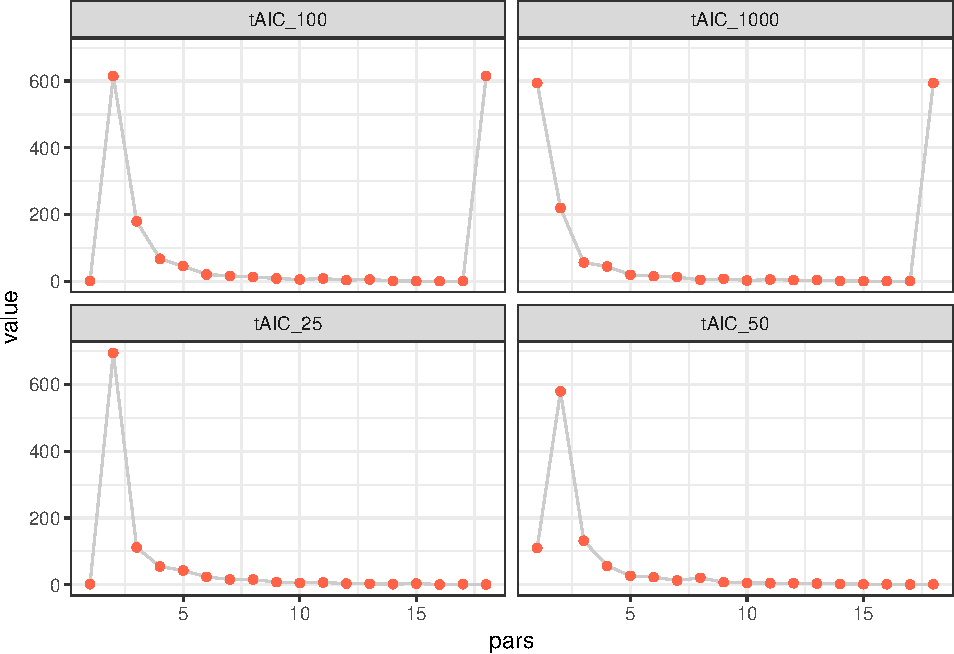
\includegraphics{exercises_files/figure-latex/unnamed-chunk-3-1.pdf}

\begin{enumerate}
\def\labelenumi{\arabic{enumi}.}
\setcounter{enumi}{1}
\tightlist
\item
  Vary the simulation, using
\end{enumerate}

\[ w(x) = \frac{1.2}{1 + exp\{-x\}},\]

to see how AIC performs when the fitted models do not include the
simulation model.

\begin{Shaded}
\begin{Highlighting}[]
\NormalTok{w <-}\StringTok{ }\ControlFlowTok{function}\NormalTok{(x)\{}
  \FloatTok{1.2} \OperatorTok{/}\NormalTok{(}\DecValTok{1} \OperatorTok{+}\StringTok{ }\KeywordTok{exp}\NormalTok{(}\OperatorTok{-}\NormalTok{x))}
\NormalTok{\}}

\NormalTok{mu <-}\StringTok{ }\ControlFlowTok{function}\NormalTok{(x) \{}
  \DecValTok{8} \OperatorTok{*}\StringTok{ }\KeywordTok{exp}\NormalTok{(}\KeywordTok{w}\NormalTok{(x))}
\NormalTok{\}}

\NormalTok{aics <-}\StringTok{ }\KeywordTok{matrix}\NormalTok{(}\DecValTok{0}\NormalTok{, }\DataTypeTok{nrow =}\NormalTok{ B, }\DataTypeTok{ncol =}\NormalTok{ pmax)}

\ControlFlowTok{for}\NormalTok{(b }\ControlFlowTok{in} \DecValTok{1}\OperatorTok{:}\NormalTok{B)\{}
  
\NormalTok{  y <-}\StringTok{ }\KeywordTok{rpois}\NormalTok{(}\DataTypeTok{n =}\NormalTok{ M }\OperatorTok{*}\StringTok{ }\NormalTok{n, }\DataTypeTok{lambda =} \KeywordTok{mu}\NormalTok{(x))}
  
\NormalTok{  mod <-}\StringTok{ }\KeywordTok{glm}\NormalTok{(y }\OperatorTok{~}\StringTok{ }\DecValTok{1}\NormalTok{, }\DataTypeTok{family =}\NormalTok{ poisson)}
\NormalTok{  aics[b, }\DecValTok{1}\NormalTok{] <-}\StringTok{ }\KeywordTok{AIC}\NormalTok{(mod)}
  
\NormalTok{  formula <-}\StringTok{ "y ~ x"}
\NormalTok{  mod <-}\StringTok{ }\KeywordTok{glm}\NormalTok{(formula, }\DataTypeTok{family =}\NormalTok{ poisson)}
\NormalTok{  aics[b, }\DecValTok{2}\NormalTok{ ] <-}\StringTok{ }\KeywordTok{AIC}\NormalTok{(mod)}
  
  \ControlFlowTok{for}\NormalTok{(j }\ControlFlowTok{in} \DecValTok{3}\OperatorTok{:}\NormalTok{pmax)\{}
\NormalTok{    formula <-}\StringTok{ }\KeywordTok{paste}\NormalTok{(formula, }\StringTok{" + I(x^"}\NormalTok{, j }\OperatorTok{-}\StringTok{ }\DecValTok{1}\NormalTok{, }\StringTok{")"}\NormalTok{, }\DataTypeTok{sep =} \StringTok{""}\NormalTok{)}
\NormalTok{    mod <-}\StringTok{ }\KeywordTok{glm}\NormalTok{(formula, }\DataTypeTok{family =}\NormalTok{ poisson)}
\NormalTok{    aics[b, j] <-}\StringTok{ }\KeywordTok{AIC}\NormalTok{(mod)}
\NormalTok{  \}}
\NormalTok{\}}

\NormalTok{AICorder <-}\StringTok{ }\KeywordTok{apply}\NormalTok{(aics, }\DecValTok{1}\NormalTok{, which.min) }\OperatorTok{-}\StringTok{ }\DecValTok{1}
\NormalTok{tAIC <-}\StringTok{ }\KeywordTok{table}\NormalTok{(AICorder)}

\NormalTok{tAIC }\OperatorTok\StringTok{ }
\StringTok{  }\KeywordTok{as.data.frame}\NormalTok{() }\OperatorTok\StringTok{ }
\StringTok{  }\KeywordTok{ggplot}\NormalTok{(}\KeywordTok{aes}\NormalTok{(AICorder, Freq, }\DataTypeTok{group =} \DecValTok{1}\NormalTok{)) }\OperatorTok{+}
\StringTok{  }\KeywordTok{geom_line}\NormalTok{(}\DataTypeTok{colour =} \StringTok{"gray80"}\NormalTok{) }\OperatorTok{+}
\StringTok{  }\KeywordTok{geom_point}\NormalTok{(}\DataTypeTok{colour =} \StringTok{"orange"}\NormalTok{) }\OperatorTok{+}
\StringTok{  }\KeywordTok{theme_bw}\NormalTok{()}
\end{Highlighting}
\end{Shaded}

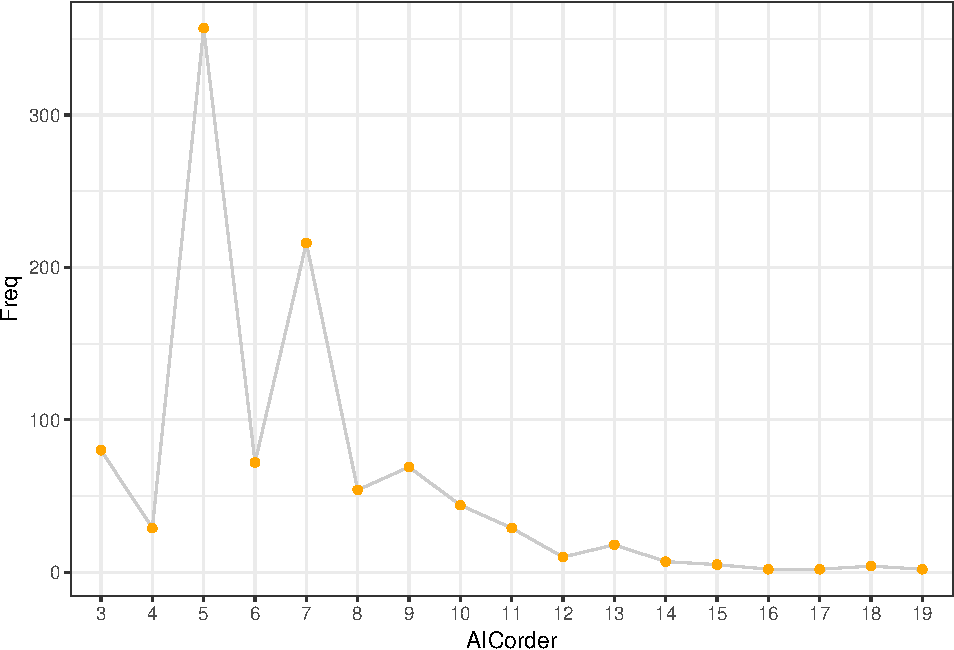
\includegraphics{exercises_files/figure-latex/unnamed-chunk-4-1.pdf}

\begin{enumerate}
\def\labelenumi{\arabic{enumi}.}
\setcounter{enumi}{2}
\tightlist
\item
  Modify the code above to compute the values of BIC and \(AIC_{c}\),
  where
\end{enumerate}

\[ AIC_{c} = AIC + \frac{2p^2 + 2p}{n - p - 1}\]

\begin{Shaded}
\begin{Highlighting}[]
\NormalTok{w <-}\StringTok{ }\ControlFlowTok{function}\NormalTok{(x)\{}
  \FloatTok{0.001} \OperatorTok{*}\StringTok{ }\NormalTok{(}\DecValTok{100} \OperatorTok{+}\StringTok{ }\NormalTok{x }\OperatorTok{+}\StringTok{ }\NormalTok{x}\OperatorTok{^}\DecValTok{2} \OperatorTok{+}\StringTok{ }\NormalTok{x}\OperatorTok{^}\StringTok{ }\DecValTok{3}\NormalTok{)}
\NormalTok{\}}

\NormalTok{mu <-}\StringTok{ }\ControlFlowTok{function}\NormalTok{(x) \{}
  \DecValTok{8} \OperatorTok{*}\StringTok{ }\KeywordTok{exp}\NormalTok{(}\KeywordTok{w}\NormalTok{(x))}
\NormalTok{\}}

\NormalTok{aics <-}\StringTok{ }\KeywordTok{matrix}\NormalTok{(}\DecValTok{0}\NormalTok{, }\DataTypeTok{nrow =}\NormalTok{ B, }\DataTypeTok{ncol =}\NormalTok{ pmax)}

\ControlFlowTok{for}\NormalTok{(b }\ControlFlowTok{in} \DecValTok{1}\OperatorTok{:}\NormalTok{B)\{}
  
\NormalTok{  y <-}\StringTok{ }\KeywordTok{rpois}\NormalTok{(}\DataTypeTok{n =}\NormalTok{ M }\OperatorTok{*}\StringTok{ }\NormalTok{n, }\DataTypeTok{lambda =} \KeywordTok{mu}\NormalTok{(x))}
  
\NormalTok{  mod <-}\StringTok{ }\KeywordTok{glm}\NormalTok{(y }\OperatorTok{~}\StringTok{ }\DecValTok{1}\NormalTok{, }\DataTypeTok{family =}\NormalTok{ poisson)}
\NormalTok{  p <-}\StringTok{ }\KeywordTok{length}\NormalTok{(mod}\OperatorTok{$}\NormalTok{coefficients) }
\NormalTok{  aics[b, }\DecValTok{1}\NormalTok{] <-}\StringTok{ }\KeywordTok{AIC}\NormalTok{(mod) }\OperatorTok{+}\StringTok{ }\NormalTok{(}\DecValTok{2}\OperatorTok{*}\NormalTok{p}\OperatorTok{^}\DecValTok{2} \OperatorTok{+}\StringTok{ }\DecValTok{2}\OperatorTok{*}\NormalTok{p)}\OperatorTok{/}\NormalTok{(n }\OperatorTok{-}\StringTok{ }\NormalTok{p }\OperatorTok{-}\StringTok{ }\DecValTok{1}\NormalTok{)}
  
\NormalTok{  formula <-}\StringTok{ "y ~ x"}
\NormalTok{  mod <-}\StringTok{ }\KeywordTok{glm}\NormalTok{(formula, }\DataTypeTok{family =}\NormalTok{ poisson)}
\NormalTok{  p <-}\StringTok{ }\KeywordTok{length}\NormalTok{(mod}\OperatorTok{$}\NormalTok{coefficients) }
\NormalTok{  aics[b, }\DecValTok{2}\NormalTok{ ] <-}\StringTok{ }\KeywordTok{AIC}\NormalTok{(mod) }\OperatorTok{+}\StringTok{ }\NormalTok{(}\DecValTok{2}\OperatorTok{*}\NormalTok{p}\OperatorTok{^}\DecValTok{2} \OperatorTok{+}\StringTok{ }\DecValTok{2}\OperatorTok{*}\NormalTok{p)}\OperatorTok{/}\NormalTok{(n }\OperatorTok{-}\StringTok{ }\NormalTok{p }\OperatorTok{-}\StringTok{ }\DecValTok{1}\NormalTok{)}
  
  \ControlFlowTok{for}\NormalTok{(j }\ControlFlowTok{in} \DecValTok{3}\OperatorTok{:}\NormalTok{pmax)\{}
\NormalTok{    formula <-}\StringTok{ }\KeywordTok{paste}\NormalTok{(formula, }\StringTok{" + I(x^"}\NormalTok{, j }\OperatorTok{-}\StringTok{ }\DecValTok{1}\NormalTok{, }\StringTok{")"}\NormalTok{, }\DataTypeTok{sep =} \StringTok{""}\NormalTok{)}
\NormalTok{    mod <-}\StringTok{ }\KeywordTok{glm}\NormalTok{(formula, }\DataTypeTok{family =}\NormalTok{ poisson)}
\NormalTok{    p <-}\StringTok{ }\KeywordTok{length}\NormalTok{(mod}\OperatorTok{$}\NormalTok{coefficients) }
\NormalTok{    aics[b, j] <-}\StringTok{ }\KeywordTok{AIC}\NormalTok{(mod) }\OperatorTok{+}\StringTok{ }\NormalTok{(}\DecValTok{2}\OperatorTok{*}\NormalTok{p}\OperatorTok{^}\DecValTok{2} \OperatorTok{+}\StringTok{ }\DecValTok{2}\OperatorTok{*}\NormalTok{p)}\OperatorTok{/}\NormalTok{(n }\OperatorTok{-}\StringTok{ }\NormalTok{p }\OperatorTok{-}\StringTok{ }\DecValTok{1}\NormalTok{)}
\NormalTok{  \}}
\NormalTok{\}}


\NormalTok{AICorder <-}\StringTok{ }\KeywordTok{apply}\NormalTok{(aics, }\DecValTok{1}\NormalTok{, which.min) }\OperatorTok{-}\StringTok{ }\DecValTok{1}
\NormalTok{tAIC <-}\StringTok{ }\KeywordTok{table}\NormalTok{(AICorder)}

\NormalTok{tAIC }\OperatorTok\StringTok{ }
\StringTok{  }\KeywordTok{as.data.frame}\NormalTok{() }\OperatorTok\StringTok{ }
\StringTok{  }\KeywordTok{ggplot}\NormalTok{(}\KeywordTok{aes}\NormalTok{(AICorder, Freq, }\DataTypeTok{group =} \DecValTok{1}\NormalTok{)) }\OperatorTok{+}
\StringTok{  }\KeywordTok{geom_line}\NormalTok{(}\DataTypeTok{colour =} \StringTok{"gray80"}\NormalTok{) }\OperatorTok{+}
\StringTok{  }\KeywordTok{geom_point}\NormalTok{(}\DataTypeTok{colour =} \StringTok{"blue3"}\NormalTok{) }\OperatorTok{+}
\StringTok{  }\KeywordTok{theme_bw}\NormalTok{()}
\end{Highlighting}
\end{Shaded}

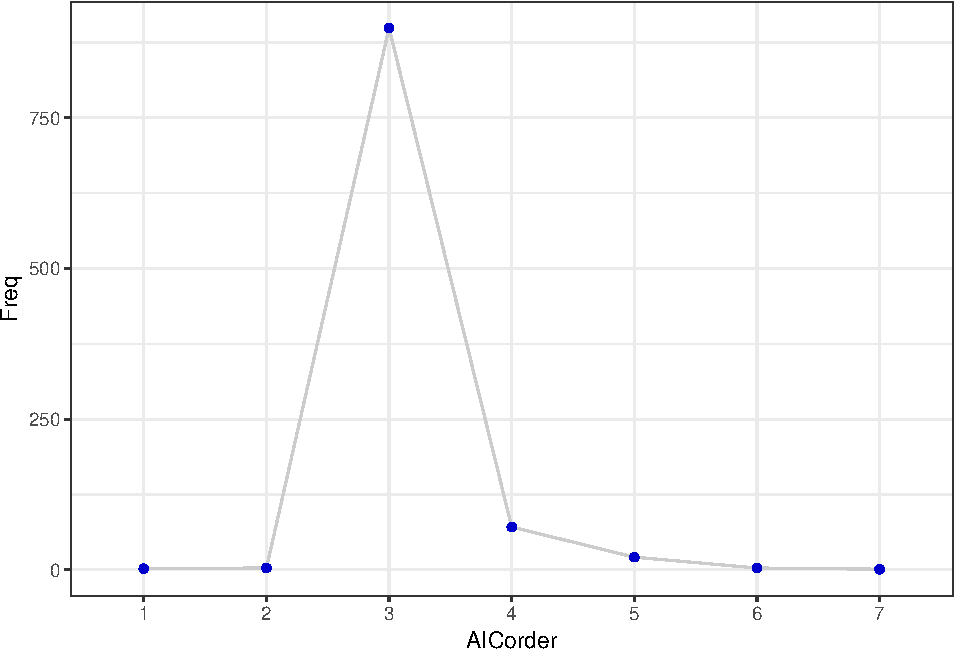
\includegraphics{exercises_files/figure-latex/unnamed-chunk-5-1.pdf}


\end{document}
